\documentclass[11pt,a4paper]{article}
\usepackage[utf8]{inputenc}
\usepackage[T1]{fontenc}
\usepackage[french]{babel}
\usepackage{lmodern}
\usepackage[margin=2.3cm]{geometry}
\usepackage{graphicx}
\usepackage{booktabs}
\usepackage{amsmath}
\usepackage{hyperref}
\graphicspath{{../figures/}}

\title{Loi d'Okun aux États-Unis : le PIB réel explique-t-il la variation du chômage ?}
\author{Fatima Zahra HAJJI \\ Sujet F16 · Machine Learning appliqué à la finance (S7 FIN et CI)}
\date{22 novembre 2026}

\begin{document}
\maketitle

\section{Problématique et objectif}
Dans quelle mesure la croissance du PIB réel permet-elle d'expliquer la variation du taux de chômage aux États-Unis ? On estime le modèle
\[
\Delta U_t = \alpha + \beta\, g_t + \varepsilon_t ,
\]
où $g_t$ est la croissance trimestrielle du PIB réel (en \%) et $\Delta U_t$ la variation trimestrielle du chômage (en points). Le coefficient d'Okun $\beta$ est attendu négatif. Critère de réussite fixé avant les résultats : battre la référence naïve (moyenne d'entraînement) en RMSE sur un test chronologique.

\section{Données}
Deux séries FRED : GDPC1 (PIB réel, BEA, trimestriel) et UNRATE (taux de chômage, BLS, mensuel, ramené au trimestre par la moyenne de trois mois). La procédure de téléchargement est décrite dans \texttt{data/raw/README.md}.

\section{Méthode}
Régression linéaire simple estimée par moindres carrés, intégrée à un \texttt{Pipeline} scikit-learn (imputation par la médiane, ajustée sur l'entraînement seul). Découpage chronologique : entraînement jusqu'à 2009~T4 (247 trimestres), validation 2010--2016 (28), test à partir de 2017~T1 (38), utilisé une seule fois après réajustement sur entraînement et validation. Graine : 42.

\begin{figure}[h]
\centering
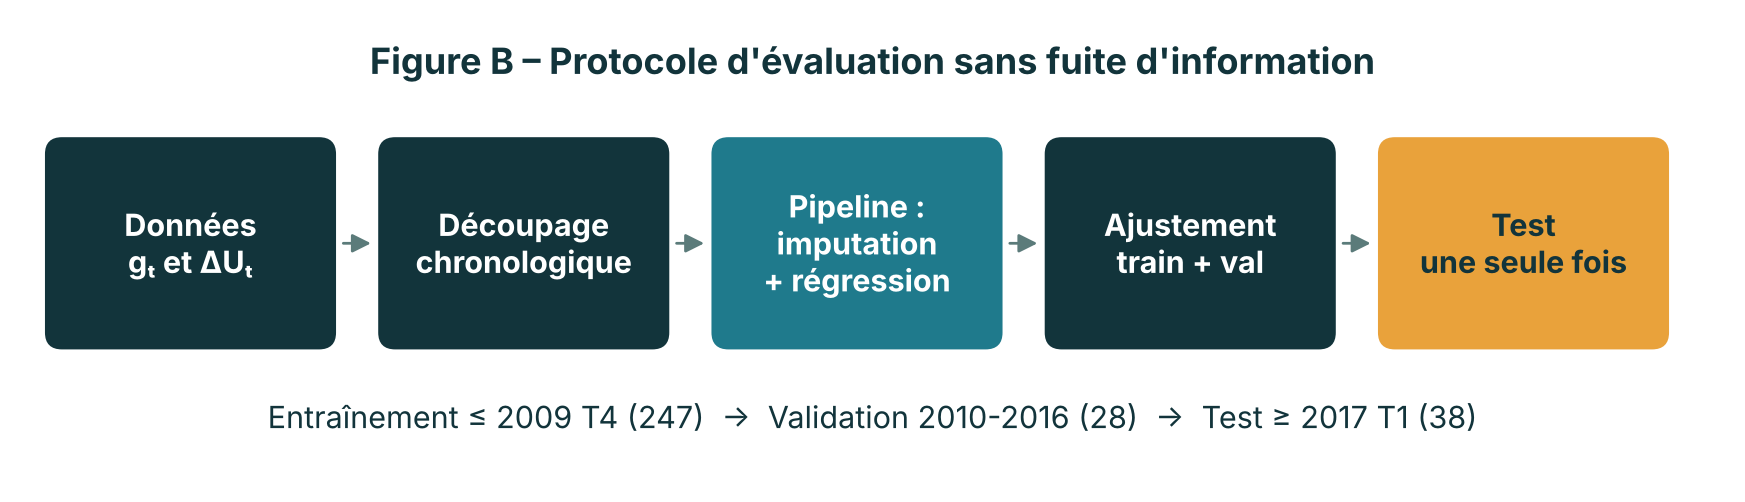
\includegraphics[width=\textwidth]{figB_protocole.png}
\caption{Protocole d'évaluation.}
\end{figure}

\section{Résultats}
\begin{table}[h]
\centering
\begin{tabular}{lcc}
\toprule
 & Régression linéaire & Référence naïve \\
\midrule
RMSE, test complet & 1,224 & 1,688 \\
RMSE, test hors 2020-2021 & 0,197 & 0,133 \\
\bottomrule
\end{tabular}
\caption{RMSE sur le jeu de test (points de pourcentage).}
\end{table}

Le coefficient estimé est $\hat\beta = -0{,}279$ (IC à 95\,\% indicatif : $[-0{,}314\,;\,-0{,}244]$), soit $-0{,}28$ point de chômage par point de croissance trimestrielle. La croissance « neutre » ($\Delta U = 0$) est d'environ $0{,}80\,\%$ par trimestre. Le $R^2$ vaut $0{,}474$ sur le test complet et $-1{,}434$ hors 2020-2021.

\begin{figure}[h]
\centering
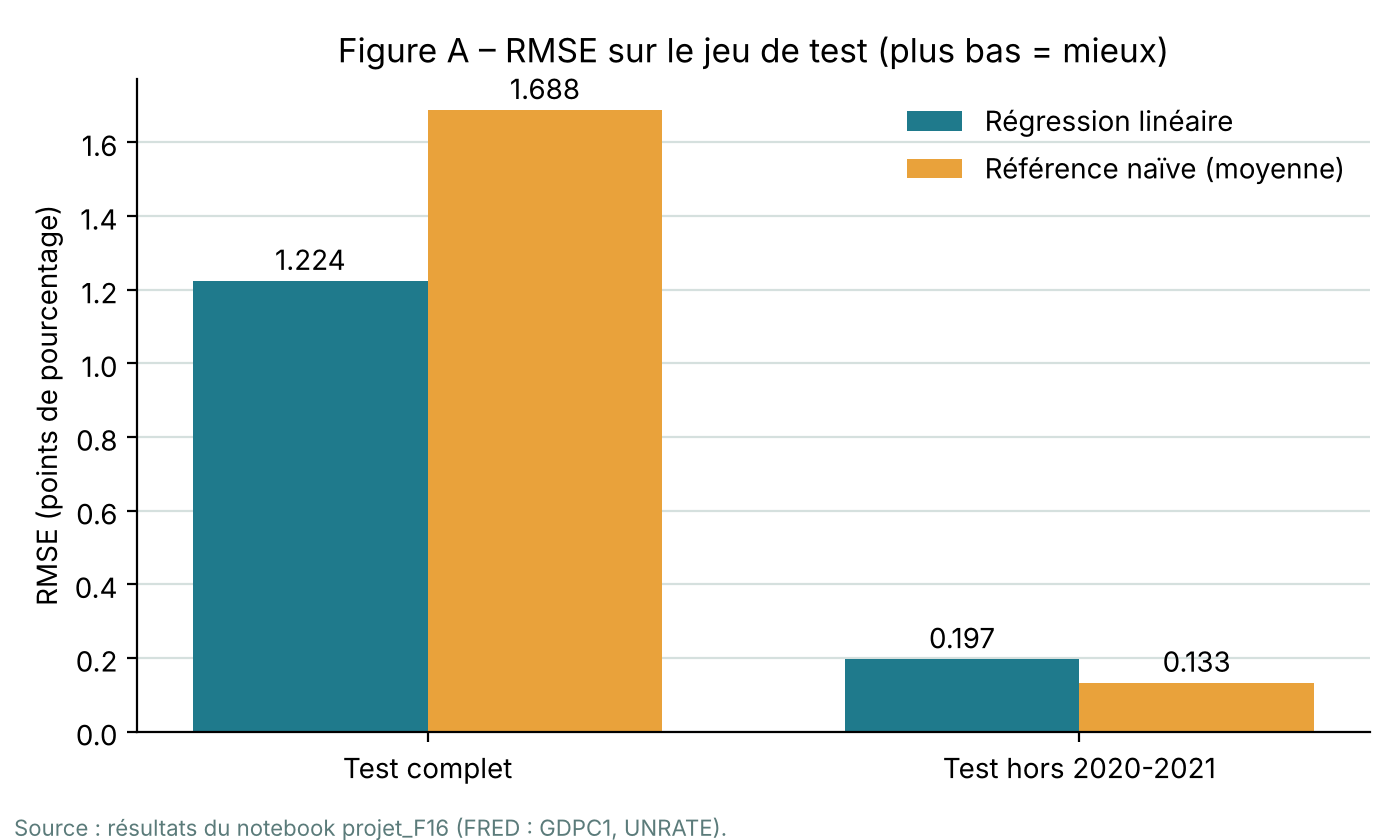
\includegraphics[width=0.8\textwidth]{figA_rmse_test.png}
\caption{RMSE de la régression et de la référence naïve.}
\end{figure}

\section{Limites et conclusion}
L'intervalle de confiance suppose des erreurs indépendantes et de variance constante, hypothèses douteuses sur des séries temporelles : il est donc probablement trop étroit. Le test complet contient le choc de 2020, qui explique l'essentiel du gain de la régression ; hors 2020-2021, la référence naïve est meilleure.

\textbf{Réponse à la problématique} : la croissance du PIB réel explique une part de la variation du chômage ($\hat\beta<0$, $R^2$ test $=0{,}47$), surtout lors des grands chocs, mais la prédiction hors échantillon reste fragile. Pistes : ajouter la croissance retardée, utiliser une régression robuste ou une indicatrice pour 2020-2021, estimer $\beta$ sur fenêtre glissante.

\section*{Références}
Okun (1962), \emph{Potential GNP: Its Measurement and Significance} ; Ball, Leigh et Loungani (2017), Okun's Law: Fit at 50?, \emph{Journal of Money, Credit and Banking} ; Pedregosa et al. (2011), Scikit-learn, \emph{JMLR} 12 ; FRED, Federal Reserve Bank of St.~Louis.

\end{document}
